%\VignetteEngine{knitr::knitr}
%\VignetteIndexEntry{Imputation Methods in robCompositions}
\documentclass{scrartcl}
\usepackage[pdftex]{hyperref}
\usepackage{amssymb, amsfonts}
%\usepackage[authoryear]{cite}
\usepackage[authoryear]{natbib}
%\usepackage{amsmath, amsfonts, amssymb} 
%\usepackage[authoryear]{natbib}
%\usepackage{graphicx,fancyhdr,vmargin}
%\usepackage{natbib}

\hypersetup{colorlinks,
        citecolor=blue,
        linkcolor=blue,
        urlcolor=blue
}

\def\R{\hbox{\znaky R}}
\def\A{\hbox{\znaky A}} \def\hA{\hbox{\hznaky A}}
\def\M{\hbox{\znaky M}}
\def\N{\hbox{\znaky N}}
\newcommand{\plural}[1]{\ensuremath{\underline{\mathbf{#1}}}}
\def\tucne#1{\mbox{\mathversion{bold}$#1$}}
\newcommand{\m}[1]{\ensuremath{\mathbf{#1}}}
%\renewcommand{\boma}[1]{\mbox{\boldmath ${#1}$}}
  
\newcommand{\Rlogo}{\raisebox{-.1mm}{\includegraphics[width=1.2em]{logo.pdf}}}
 
\begin{document}



\begin{flushleft}
  {\LARGE\textbf{Robust Imputation of Missing
  Values in} \\[2mm]  \vspace*{-0.8cm} \textbf{Compositional Data Using the\Rlogo-Package} 
  \vspace*{0.55cm} \texttt{robCompositions}}
  \vspace{1.0cm}
  
  Matthias Templ$^{*,**}$, Peter Filzmoser$^{*}$, Karel Hron$^{***}$
  
{\small
\begin{description}
\item $^{*}\;$  Department of Statistics and Probability Theory, Vienna
University of Technology, Wiedner Hauptstr. 8-10, 1040 Vienna, Austria.
(\href{templ@tuwien.ac.at}{templ@tuwien.ac.at}) \\
\item $^{**}\;$    Department of Methodology, Statistics Austria, Guglgasse 13,
1110 Vienna, Austria.
(\href{matthias.templ@statistik.gv.at}{matthias.templ@statistik.gv.at}) and \\
\item $^{***}\;$ Department of Mathematical Analysis and Applications of
Mathematics, Palack\'y University, Tomkova 40, 779 00 Olomouc, Czech Republic. 
  (\href{hronk@seznan.cz}{hronk@seznan.cz})
\end{description}
}
\end{flushleft}
\vspace{1cm}



\begin{center} {\large Abstract} \end{center}

\abstract{The aim of this contribution is to show how the R-package
\texttt{robCompositions} can be applied to estimate missing values in
compositional data. Two procedures are summarized, one of them being
highly stable also in presence of outlying observations.
Measures for information loss are presented, and it is demonstrated
how they can be applied. Moreover, we introduce new diagnostic tools
that are useful for inspecting the quality of the imputed data.}


%%%%%%%%%%%%%%%%%%%%%%%%%%%%%%%%%%%%%%%%%%%%%%
\section{Introduction}


\subsection{Imputation}
Many different methods for imputation have been developed over the last few decades.
The techniques for imputation can be subdivided into four categories: univariate methods 
such as column-wise (conditional) mean or median imputation, distance-based imputation 
methods such as $k$-nearest neighbor imputation, covariance-based methods such as the 
well-known expectation maximization imputation method, and model-based methods such as 
regression imputation. 
%If an algorithm includes a certain kind of randomness it may be 
%adapted for multiple imputation.
Most of these methods are able to deal with missing completely at random (MCAR) 
and missing at random (MAR) missing values mechanism (see, e.g.
\cite{Little87}). However, most of the existing methods assume that the data originate 
from a multivariate normal distribution. 
This assumption becomes invalid as soon as there are outliers in the data. In that case
imputation methods based on robust estimates should be used.


\subsection{Compositional Data}

Advanced (robust) imputation methods have turned out to work well for data
with a direct representation in the Euclidean space. However, this is not 
the case when dealing with compositional data.

An observation
$\m{x}=(x_1,\dots,x_D)$ is called a $D$-part composition
if, and only if, all its components are strictly positive real numbers and all
the relevant information is included in the ratios between them
\citep{Aitchison86}.
One can thus define the \textit{simplex}, which is the sample space of $D$-part
compositions, as 
\begin{equation}
\mathcal{S}^D=\{\m{x}=(x_1,\dots,x_D),\,x_i> 0,\,\sum_{i=1}^Dx_i=\kappa\} \ \ .
\end{equation}
Note that the constant sum constraint $\kappa$ implies that $D$-part
compositions are only $D-1$ dimensional, so they are singular by definition.
It is, however, possible that the constant $\kappa$ is different for
each observation (for further details, see \cite{Hron09}). 
In any case, the important property of compositional data is that all information is 
contained in the ratios of the parts.

The application of standard statistical methods, like correlation analysis or principal 
component analysis, directly to compositional data can lead to biased and meaningless 
results \citep{Filzmoser08a, Filzmoser08b}. This is also
true for imputation methods \citep{bren08, Fern03, Boogaart06}.
A way out is to first transform the data with appropriate transformation methods.
Such transformations, preserving the specific geometry of compositional data on
the simplex (also called Aitchison geometry), are represented by the family of log-ratio
transformations: additive, centered \citep{Aitchison86} and isometric
(abbreviated by \textit{ilr}, \citep{Egozcue03} transformations.
Standard statistical methods can then be applied to the transformed data, and
the results can be back-transformed.

Compositional data frequently occur in official statistics. Examples are expenditure 
data, income components in tax data, wage components in the Earnings Structure Survey, 
components of turnover of enterprises etc., and all data which sum up to a
constant or which carry all the information only in the ratios.
The problem of missing values in compositional data including outliers is a common
problem not only in official statistics, but also in various other fields 
(see, e.g., \citep{Graf06, Filzmoser08a}).
In the following Section we will briefly review two algorithms for imputation
that are described in detail in \cite{Hron09}. Section 3 focuses on the 
use of the R-package \texttt{robCompositions}, and Section 4 introduces
some diagnostic tools implemented in this package. The final Section 5 concludes.


\section{Proposed Imputation Algorithms}

In the following we briefly describe the imputation methods that have been 
implemented in the R-package \texttt{robCompositions}. The 
detailed description of the algorithms can be found in \cite{Hron09}. 

\subsection{$k$-Nearest Neighbor Imputation}

$k$-nearest neighbor imputation usually uses the Euclidean distance
measure. Since compositional data are represented only in the simplex sample
space, we have to use a different distance measure, like the 
Aitchison distance, being
defined for two compositions $\m{x}=(x_1,\dots,x_D)$ and $\m{y}=(y_1,\dots,y_D)$ as
\begin{equation}
\label{adist}
d_a(\m{x},\m{y})=\sqrt{\frac{1}{D}\sum_{i=1}^{D-1}\sum_{j=i+1}^D
\left(\ln\frac{x_i}{x_j}-\ln\frac{y_i}{y_j}\right)^2} .
\end{equation}  
Thus, the Aitchison distance takes care of the property that compositional data
include their information only in the ratios between the parts.

Once the $k$-nearest neighbors to an observation with missing parts have been
identified, their information is used to estimate the missings. For reasons
of robustness, the estimation is based on using medians rather than means.
If the compositional
data do not sum up to a constant, it is important to use an adjustment according
the sum of all parts prior to imputation. For details, see \cite{Hron09}.


\subsection{Iterative Model-Based Imputation}

In the second approach we initialize the missing values with the proposed $k$-nearest 
neighbor approach. Then the data are transformed to the
$D-1$ dimensional real space using the ilr transformation.
Let $d_e$ denote the Euclidean distance. The ilr transformation holds the
so-called isometric property,
\begin{equation}
d_a(\m{x},\m{y})=d_e(ilr(\m{x}),ilr(\m{y})) 
\end{equation}
\citep{Egozcue05}. Consequently, one can use standard statistical methods 
like multiple linear regression, that work correctly in the Euclidean space.

We take a special form of the ilr transformation, namely
$ilr(\m{x})=(z_1,\dots,z_{D-1})$, with 
\begin{equation}
z_i=\sqrt{\frac{D-i}{D-i+1}}\,\ln\frac{\sqrt[D-i]{\prod_{j=i+1}^Dx_j}}{x_{i}}
\quad \mbox{ for } i=1,\ldots ,D-1 \ \ .
\end{equation}
Here, the compositional part $x_1$ includes the highest amount of missings,
$x_2$ the next highest, and so on. Thus, when performing a regression of 
$z_1$ on $z_2,\dots, z_{D-1}$, only $z_1$ will be influenced by the initialized
missings in $x_1$, but not the remaining ilr variables.

The idea of the procedure is thus to iteratively improve the estimation of the
missing values. After the regression of $z_1$ on $z_2,\dots, z_{D-1}$, the
results are back-transformed to the simplex, and the cells that were originally missing 
are updated. 
Next we consider the variable which originally has the second highest amount
of missings, and the same regression procedure as before is applied in the
ilr space. After each variable containing missings has been proceeded,
one can start the whole process again until
the estimated missings stabilize.
The detailed description of this algorithm can be found in \cite{Hron09}.

As a regression method we propose to use robust regression, like LTS regression
(see \cite{Maronna06}), especially if outliers might be present in the data.


\section{Using the R-package \texttt{robCompositions} for Imputing Missing Values}

%\subsection{Data Sets in the Package}
%
%Three data sets are included in the package, namely

%<<data sets>>=
%library(robCompositions)
%data(aitchison359)
%data(aitchison360)
%data(aitchison395)
%@
%
%These data sets can be found in the book from \cite{Aitchison86} on page 359,
%360 and 395.
%
%In the following we will use the aitchison395 data set which consists
%of household expenditures on five commodity groups of 20 single men. The
%variables represent housing (including fuel and light), foodstuff, alcohol and tobacco, 
%other goods (including clothing, footwear and durable goods) and services 
%(including transport and vehicles). Thus they represent
%the ratios of the men's income spent on the mentioned expenditures.
%
%For further proceeding we set some values to missing which then will be imputed
%with our proposed methods.
%
%<<aitchison395>>=
%x <- aitchison395
%x[1,3] <- x[2,4] <- x[3,3] <- x[3,4] <- NA
%@

\subsection{Data}

The package includes the three compositional data sets \textit{aitchison359},
\textit{aitchison360}, and \textit{aitchison395}, that have been published
in \cite{Aitchison86}. In the following, however, we will use simulated data,
where the data structure and outliers are exactly known.
The data generation is the same as described in \cite{Hron09}, and
a plot of the data set in shown in Figure \ref{repFig1} for the original
data (left) and for the ilr transformed data (right): We took 90 
observations with 3 parts that are normally distributed on the simplex
(i.e. they are multivariate normally distributed in the 2-dimensional
ilr space). A group of 5 outliers (\textit{group 1}) 
is added (green crosses in Figure \ref{repFig1})
that are potential outliers in the Aitchison and in the Euclidean space.
Another group (\textit{group 2}) of 5 outliers (blue triangles in Figure \ref{repFig1})
is only affecting the Euclidean space. Note that both types of outliers are
simulated to have a considerably higher sum of their parts, which is not visible
in the ternary diagram \citep{Aitchison86} in Figure \ref{repFig1} (left) where the parts
are re-scaled to have sum 1.

The generated (complete) data are stored in the list element \texttt{z2}
of object $x$. Among the non-outliers we set 20\% of the values in the first
part, 10\% in the second, and 5\% in the third part to missing, using an
MCAR mechanism. The new data set is stored in the list element \texttt{zmiss} of object $x$.

%% original:


%% neu:

 



\begin{knitrout}
\definecolor{shadecolor}{rgb}{0.969, 0.969, 0.969}\color{fgcolor}\begin{kframe}


{\ttfamily\noindent\color{warningcolor}{\#\# Warning: 'isomLRinv' is deprecated.\\\#\# Use 'pivotCoordInv' instead.\\\#\# See help("{}Deprecated"{})}}\end{kframe}
\end{knitrout}



\setkeys{Gin}{width=0.9\textwidth}
\begin{figure}[h]
\begin{center}
\vspace*{-3cm}
%<<plot-acomp, fig=TRUE, echo=FALSE>>=
%par(mfrow=c(1,2), mar=c(3.5,0,0,0))
%plot.acomp(acomp(x$z2), col=c(rep(1,90), rep(4,5), rep(3,5)), pch=c(rep(20,90), rep(2,5), rep(4,5)), cex=c(rep(0.6,90), rep(0.9,5), rep(0.9,5)))
%par(mar=c(3.5,4,0,0.1))
%plot(ilr(x$z2), col=c(rep(1,90), rep(4,5), rep(3,5)), pch=c(rep(20,90),
%rep(2,5), rep(4,5)), xlab=expression(z[1]), ylab=expression(z[2]), cex.lab=1.5, cex=c(rep(0.6,90), rep(0.9,5), rep(0.9,5))) 
%@
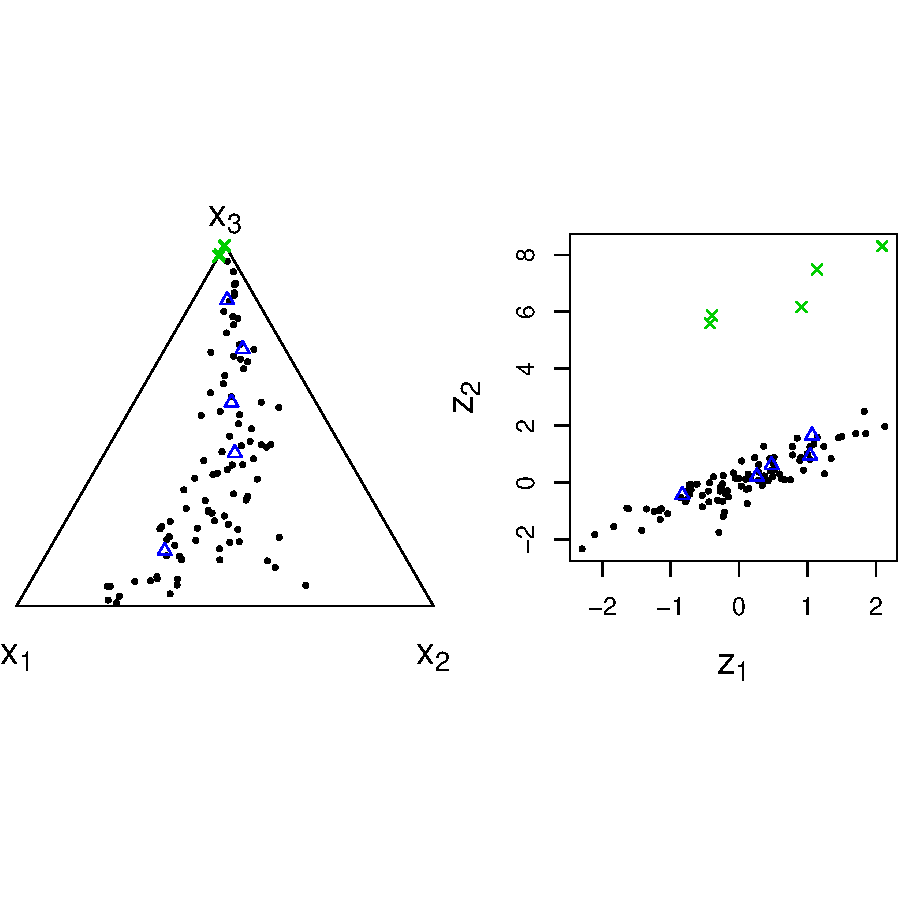
\includegraphics{plot-acomp}  
\vspace*{-33mm}
\caption{Simulated data set with 5 points from
\textit{outlier group 1} (symbol \textcolor{green}{$\times$}) 
and 5 points from \textit{outlier group 2} 
(symbol \textcolor{blue}{$\triangle$}).
Left plot: 3-part compositions shown in the ternary diagram;
right plot: data after ilr transformation.}
\label{repFig1}
\end{center}
\end{figure}



\subsection{Usage of the Imputation Methods Within the Package}


%A choice of methods is applied within the following lines of code:

%% real data set example:
%<<Imputation>>=
%xi1 <- impKNNa(x, k=4, metric="Aitchison")
%xi2 <- impKNNa(x, k=4, agg = "mean")
%xi3 <- impCoda(x, method="ltsReg", eps=0.01)
%xi4 <- impCoda(x, method="lm")
%xi5 <- impCoda(x, method="classical")
%@
%
%So, $k$-nearest neighbor imputation was performed (with aggregating
%the $k$-nearest neighbors for impuation with the median (\texttt{xi1}) and with
%the mean (\texttt{xi2}).
%In addition to that, our proposed iterative algorithms performed out,
%``ltsReg'' for robust iterative model based imputation (\texttt{xi3}), ``lm''
%for iterative model based imputation using least squares regressions
%(\texttt{xi4}), and by applying principal component analysis in an iterative
%way (\texttt{xi5}).
%
%Note that various other choices of methods and parameters can be chosen.
%
%The resulting objects (\texttt{xi1} - (\texttt{xi5}) are of class
%<<classes>>=
%class(xi1)
%@
%
%A print, a summary and a plot method are provided for objects of this class:
%<<printSummary>>=
%methods(class = "imp")
%xi1
%@
%
%All the resulting objects (\texttt{xi1} - \texttt{xi5}) return the same
%information, which can be accessed easily.
%<<names>>=
%names(xi1)
%xi1$xImp[1,3]
%@
%
%The original data set which includes the missing values is stored
%in the list element \texttt{xOrig}, the imputed data set in \texttt{xImp}. 
%In addition to that,
%the amount of missing values in the original data set is stored in the list element 
%\texttt{w} and the indices of the missing values (and therefore also of the imputed
%values) are stored in \texttt{wind}.
%All these informations are needed in order to provide suitable summaries and
%diagnostic plots.





%%%%%%%%%%%%%%%%%%%%%%%%%%%%%%%%%%%%%%%%%%%%%%%%%%%%%%%%%%%%%%%%%%%%%%%%%%%%%%%


We apply $k$-nearest neighbor imputation for the generated compositional data
set, and use the parameter $k=6$:

\begin{knitrout}
\definecolor{shadecolor}{rgb}{0.969, 0.969, 0.969}\color{fgcolor}\begin{kframe}
\begin{alltt}
\hlkwd{library}\hlstd{(}\hlstr{"robCompositions"}\hlstd{)}
\hlkwd{packageDescription}\hlstd{(}\hlstr{"robCompositions"}\hlstd{)}\hlopt{$}\hlstd{Version}
\end{alltt}
\begin{verbatim}
## [1] "2.0.3"
\end{verbatim}
\begin{alltt}
\hlstd{xImp} \hlkwb{<-} \hlkwd{impKNNa}\hlstd{(x}\hlopt{$}\hlstd{zmiss,} \hlkwc{k}\hlstd{=}\hlnum{6}\hlstd{)}
\end{alltt}
\end{kframe}
\end{knitrout}

As a default, Aitchison distances are used for identifying the $k$-nearest neighbors
(further options are provided, see help file). By default, the median is
taken for re-scaling the $k$-nearest neighbors for imputation, but also other
choices are possible.

The resulting object \texttt{xImp} is of class
\begin{knitrout}
\definecolor{shadecolor}{rgb}{0.969, 0.969, 0.969}\color{fgcolor}\begin{kframe}
\begin{alltt}
\hlkwd{class}\hlstd{(xImp)}
\end{alltt}
\begin{verbatim}
## [1] "imp"
\end{verbatim}
\end{kframe}
\end{knitrout}

A print, a summary, and a plot method are provided for objects of this class:
\begin{knitrout}
\definecolor{shadecolor}{rgb}{0.969, 0.969, 0.969}\color{fgcolor}\begin{kframe}
\begin{alltt}
\hlkwd{methods}\hlstd{(}\hlkwc{class} \hlstd{=} \hlstr{"imp"}\hlstd{)}
\end{alltt}
\begin{verbatim}
## [1] plot    print   summary
## see '?methods' for accessing help and source code
\end{verbatim}
\begin{alltt}
\hlstd{xImp}
\end{alltt}
\begin{verbatim}
## 
##  --------------------------------------- 
## [1] "31 missing values were imputed"
##  ---------------------------------------
\end{verbatim}
\end{kframe}
\end{knitrout}

Various informations are included in the object \texttt{xImp}, which can be accessed easily:

\begin{verbatim}
names(xImp)

[1] "xOrig"    "xImp"     "criteria" "iter"     "w"
"wind" "metric"
\end{verbatim} 

The list element \texttt{xOrig} contains the original data, \texttt{xImp}
is the imputed data set, \texttt{w} contains the number of missing values,
and \texttt{wind} includes the indices of the missing values
(imputed values).
All this information is needed in order to provide suitable summaries and
diagnostic plots.

\medskip
The iterative model-based imputation method is applied with:




















